\section{Durchführung}
\label{sec:Durchführung}
Zu Beginn werden die verwendeten Stäbe ausgemessen. Hierbei wird die Länge, der
Durchmesser sowie das Gewicht notiert.
In folgender Abbildung \ref{fig:aufbau} ist der Aufbau des Versuches schematisch dargestellt.
\begin{figure}[H]
  \centering
  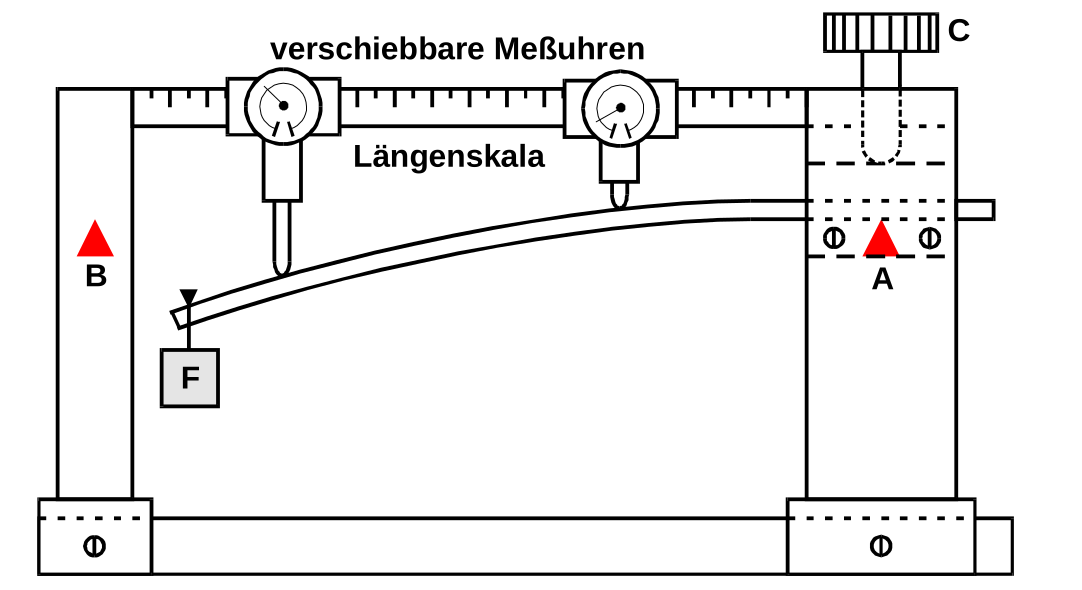
\includegraphics[scale=0.4]{content/versuchsaufbau.png}
  \caption{Schematischer Aufbau der verwendeten Apparatur.}
  \label{fig:aufbau}
\end{figure}
\noindent
Hierbei können die Probenstäbe entweder einseitig oder beidseitig eingespannt
werden. Es gibt zwei Auflagepunkte, von denen der Auflagepunkt \textbf{A} eine
Spannvorrichtung besitzt, um den Stab einseitig einspannen zu können.
Die Gewichte werden bei einseitiger Einspannung an das nicht eingespannte
Ende gehängt, bei beidseitiger Einspannung wird das Gewicht bei $x = L/2$ befestigt.
Die Durchbiegung des Stabes kann mithilfe der beiden beweglichen Messuhren ermittelt werden.
Die Messuhren besitzen eine Mikrometer-Skala und werden auf einer Millimeter-Skala positioniert.
Die Gewichte werden so gewählt, dass die maximale Durchbiegung zwischen $\SI{3}{\milli\meter}$ bis
$\SI{7}{\milli\meter}$ liegt.
